\section{Vehicle description}
The track vehicle provided for the project can be seen on \figref{TrackedVehicle} in \secref{PrototypeConstraints}. A platform of the same size of the vehicle  is mounted on the vehicle. This is to protect the servo and the mechanical system and to support the system, which include PCB boards, the battery, and the sensors used to control the vehicle. When the platform is mounted on, the vehicle is 45 cm long, 29 cm in width, 12 cm in height and it weighs 2932 grams.
The following sections will analyse the vehicle mechanical system and the features that the vehicle use to drive and steer.

\subsection{Drivetrain}

The drivetrain of a motored vehicle, is the components that transfer the rotational energy from the motor to the driving wheel of the vehicle. For this vehicle, the drivetrain will contain the gear connected to the motor, the differential gear box and the gears connected to the belts. The drivetrain is shown on \figref{vehicleDescriptionDriveTrain}.

\begin{figure}[H]
	\centering
	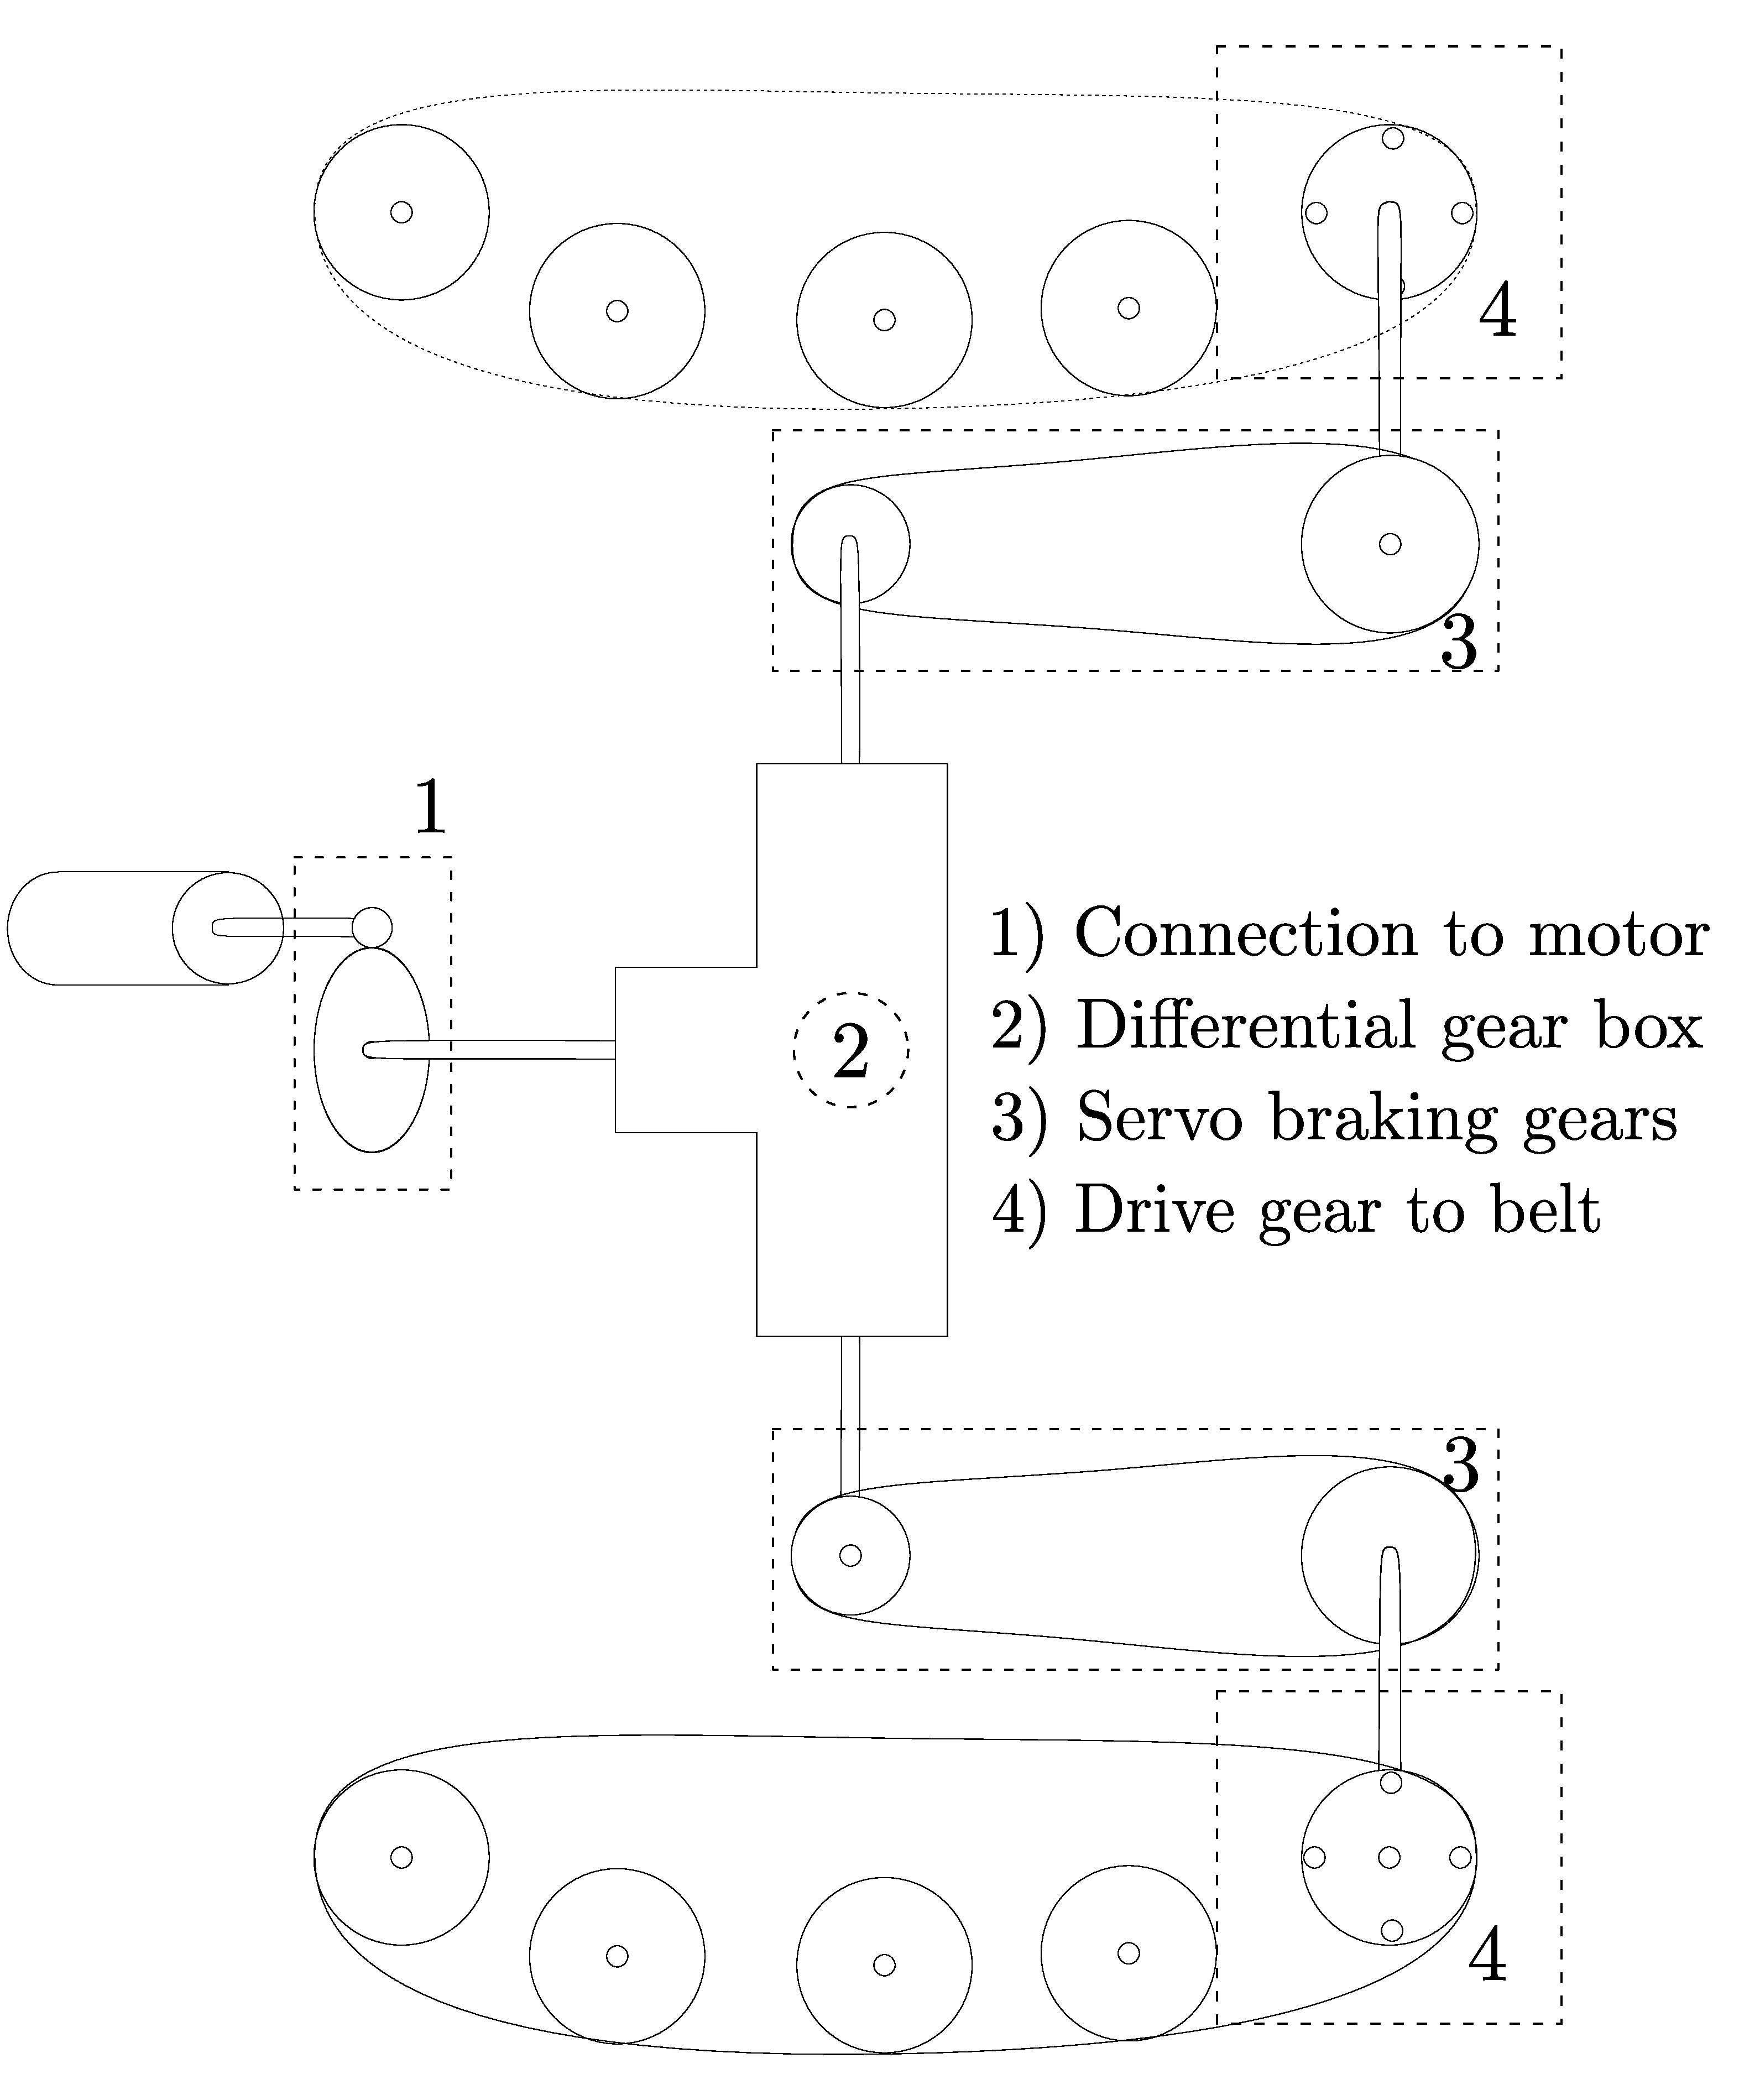
\includegraphics[scale=0.2]{figures/vehicleDescriptionDriveTrain.pdf}
	\caption{Illustration of the drive train of the vehicle.}
	\label{vehicleDescriptionDriveTrain}
\end{figure}

The motor apply a force to the system at the start of the drivetrain(1). The gear that is connected to the motor, is also connected to the differential gear box(2). The servo stands for the steering, by applying a breaking force on the breaking gears(3). The rotational energy that is that is been break for on one side, is apply on the other side, by going through the differential gear box(2). The vehicle run on two belts, that enveloping 4 wheels, plus a gear connected to the drivetrain(4). A Hall sensor is setup at each gear wheel at the track(4), to measure the speed of each belt.\\
The following sections will describe the different parts of the drivetrain seen on \figref {vehicleDescriptionDriveTrain}.\\